\section{Plugins}
\label{implementation:plugins}

Now, we will describe the implementation of a few plugins.
We implemented an infrastructure plugin that can create and remove EC2 instances in Amazon's cloud.
We created a connection plugin that allows the bootware to connect to a remote system via SSH and then execute commands on, or upload files to this system.

\subsection{AWS EC2 Plugin}

This infrastructure plugin allows the bootware to create and remove EC2 instances in Amazon's cloud.
It uses the AWS SDK for Java\footnote{\url{http://aws.amazon.com/sdkforjava/}} to implement this functionality.
This SDK specifies a specific set of action that have to be taken to start an EC2 instance, which we map onto the operations defined by each infrastructure plugin, i.e. init, shutdown, deploy, and undeploy, as described in \autoref{design:plugins}.
\autoref{image:awsplugin} shows a simplified overview of these actions and how they map onto the infrastructure plugin operations.

\begin{figure}[!htbp]
	\centering
	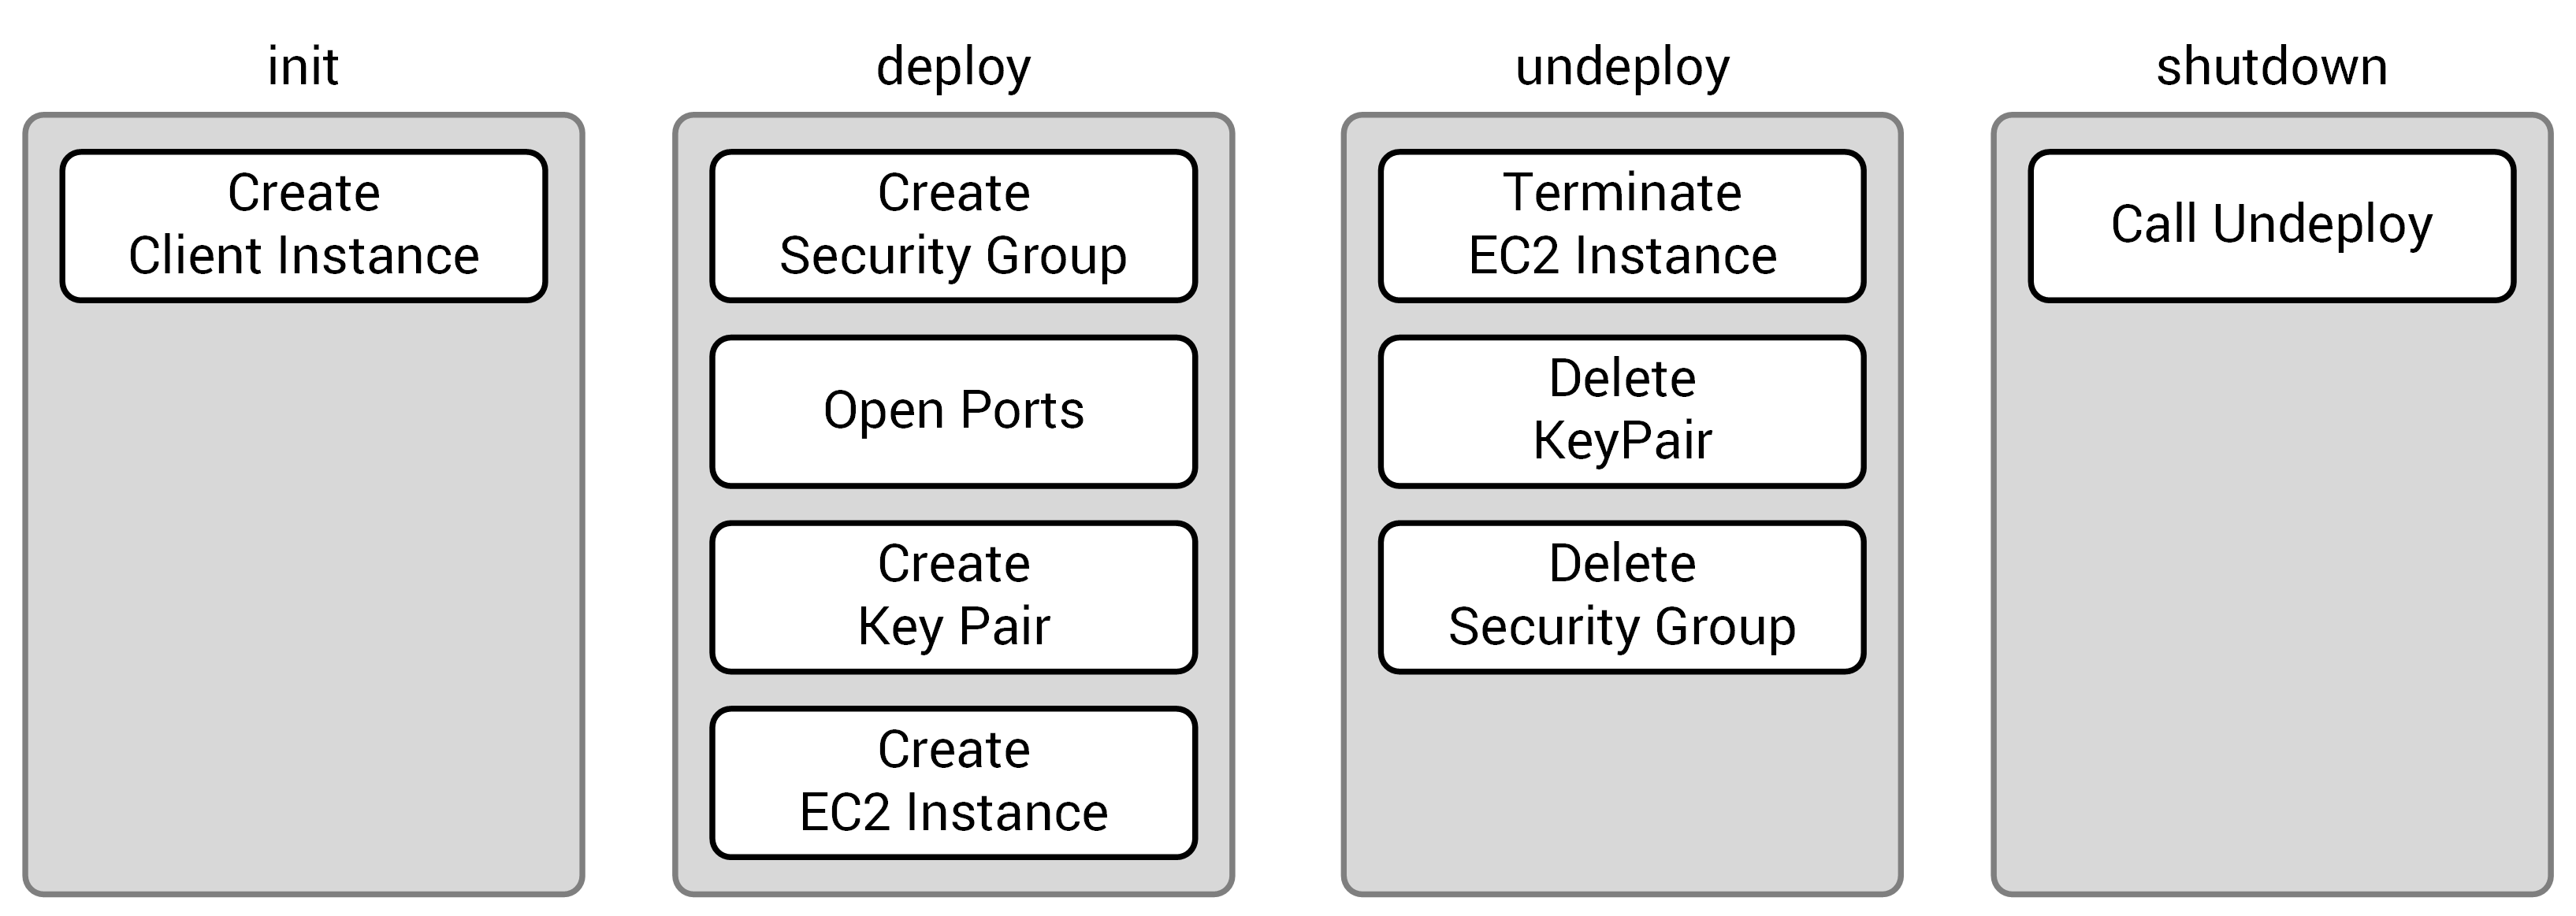
\includegraphics[resolution=600]{implementation/assets/aws_plugin}
	\caption{The operations implemented by the AWS EC2 plugin.}
	\label{image:awsplugin}
\end{figure}

The init operation, shown on the left of \autoref{image:awsplugin}, which is called once when the plugin is loaded, creates a client instance, which is an object on which all the following actions will be called.
The client instance is bound to a specific AWS region, which is read from the configuration object that is passed into the init operation.

As we can see in the deploy operation in \autoref{image:awsplugin}, we first have to create a security group\footnote{\url{http://docs.aws.amazon.com/AWSEC2/latest/UserGuide/using-network-security.html}}.
Security groups are essentially virtual firewalls that allow or deny traffic to and from all EC2 instances associated with it.
EC2 instances have to be associated with a security group, so we have to create one.
In the next step we open all ports in this security group that we later want to use for communication.
Which ports we open is determined by reading the configuration object.
We also have to create a SSH key pair and retrieve the private key, which we later use when we connect to this EC2 instance via SSH.
In the last step we create the actual EC2 instance.
Once it is up and running, the deploy operation is finished and returns an instance object which contains the URL where the EC2 instance can be reached, as well as the private key for SSH access.

The undeploy operation reverses the deploy operation.
First, it terminates the EC2 instance.
Once the instance is stopped, the key pair and the security group that were created earlier are removed.
We don't have to close the ports we opened, since they are part of the security group and don't exist anymore once the security group is removed.
After this, the EC2 instance created earlier is successfully removed.
There are no further actions necessary during the shutdown operation, but for safety we call the undeploy operation, in case it wasn't called earlier.

\subsection{SSH Plugin}

This connection plugin allows the bootware to connect to a remote system via SSH.
It uses the Ganymed SSH-2 library\footnote{https://code.google.com/p/ganymed-ssh-2/}, which implements the SSH-2 protocol in Java.
\autoref{image:sshplugin} shows a simplified overview of the actions necessary to create a SSH connection and how they map onto the connection plugin operations.

\begin{figure}[!htbp]
	\centering
	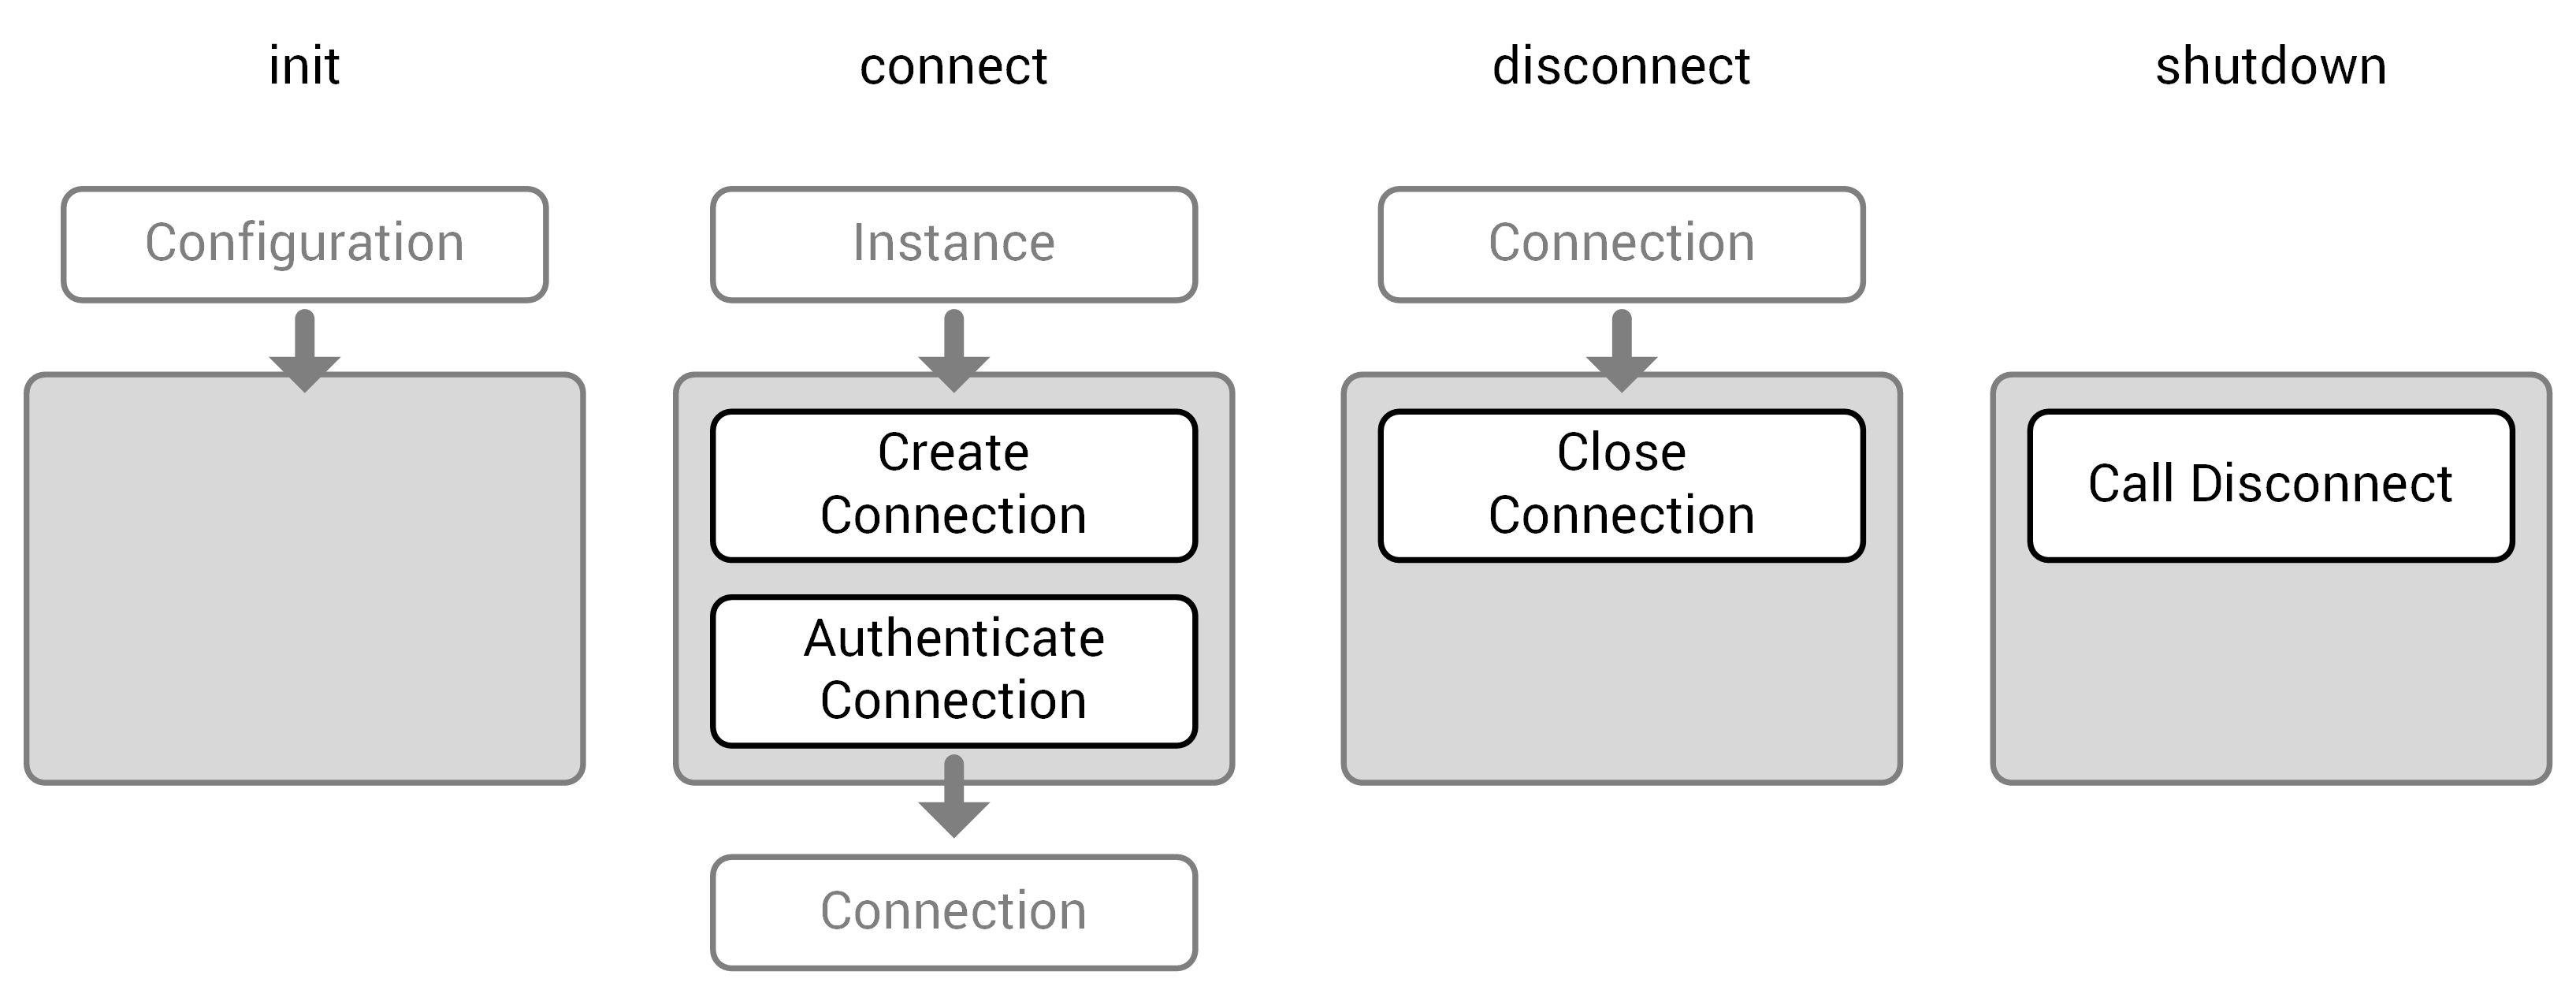
\includegraphics[resolution=600]{implementation/assets/ssh_plugin}
	\caption{The operations implemented by the SSH plugin.}
	\label{image:sshplugin}
\end{figure}

No actions are taken in the init operation.
During the connect operation, we first have to create a connection object, which is bound to a certain host name, i.e. the IP address of the remote system that we want to connect to.
We get this address from the instance object passed into the connect operation.
Then we have to authenticate this connection.
Multiple authentication methods are supported by SSH-2 protocol, including password and public key authentication.
The necessary values for these authentication methods are read from the instance object passed into the connect operation.
Once the connection is authenticated, a connection object is returned, which supports the execute and upload operation that other components can use.

The disconnect operation simply closes the connection associated with the connection object that is passed into it.
The disconnect operation is also called by the shutdown operation at the end of the plugin life cycle to close any connection that might still be open.

\subsection{OpenTOSCA Plugin}

This payload plugin allows the bootware to install an OpenTOSCA container on an EC2 instance.
It executes the installation steps described in the OpenTOSCA manual over a connection provided by a connection plugin.
\autoref{image:opentoscaplugin} shows a simplified overview of the steps involved in the installation of OpenTOSCA and how they map onto the payload plugin operations.

\begin{figure}[!htbp]
	\centering
	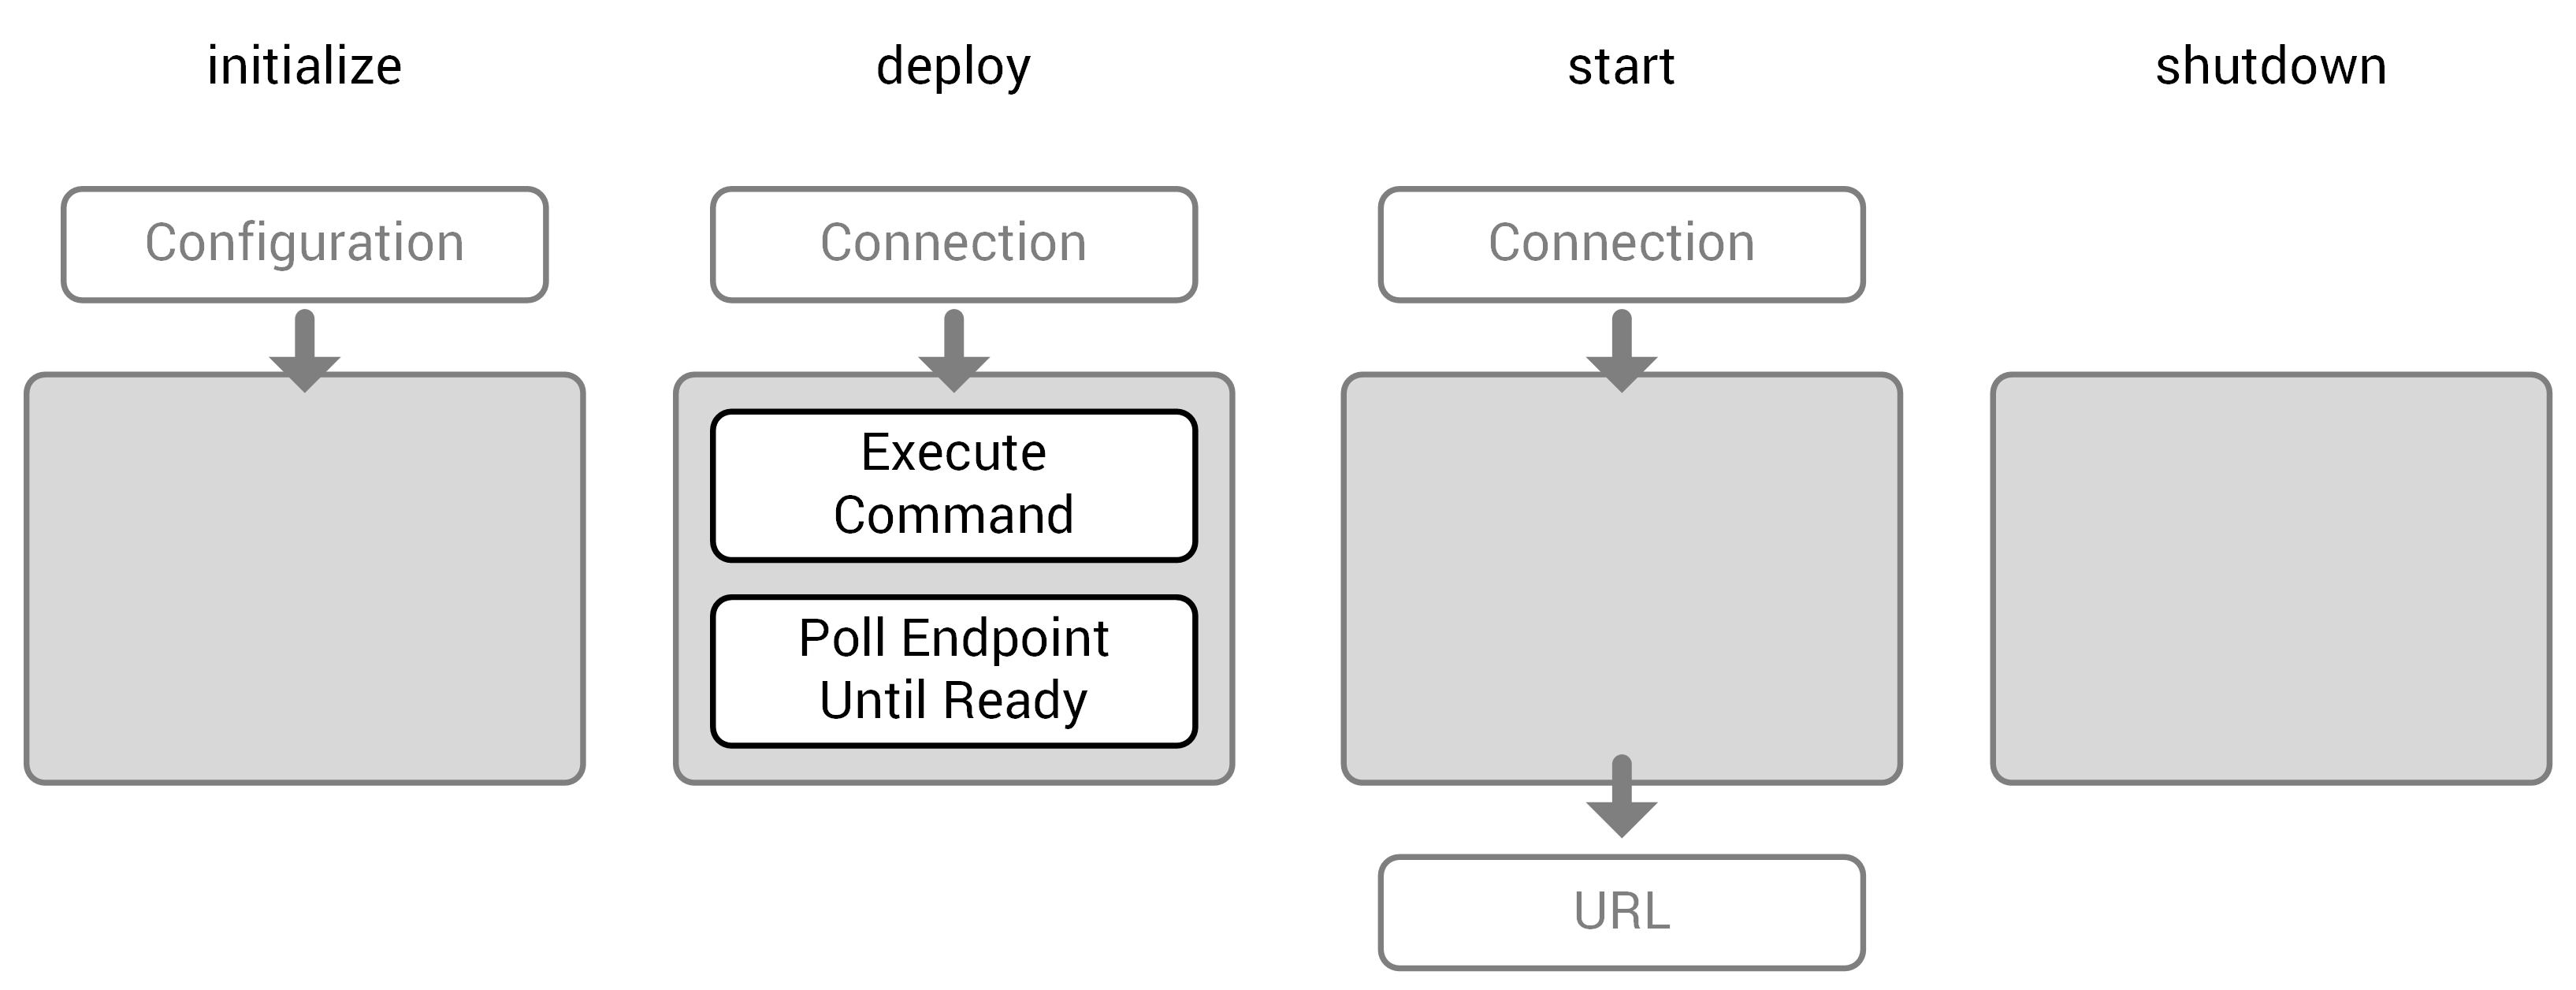
\includegraphics[resolution=600]{implementation/assets/opentosca_plugin}
	\caption{The operations implemented by the OpenTOSCA plugin.}
	\label{image:opentoscaplugin}
\end{figure}

The setup procedure for OpenTOSCA is very simply.
Only one command has to be executed over ssh, which will automatically download and install all necessary components.
After that, port 8080 on the EC2 instance is polled periodically until a connection is possible, which means that the installation process is finished.
